\title{A Note on C.P. Ramanujam}
\markright{A Note on C.P. Ramanujam}

\author{By~ S. Ramanan}
\markboth{S. Ramanan}{A Note on C.P. Ramanujam}

\date{}
\maketitle

\setcounter{page}{13}
\setcounter{pageoriginal}{10}
For\pageoriginale sheer elegance and economy, I have come across few 
mathematicians who were C.P. Ramanujam's equal. He made so many 
remarks which clarified and threw light on different branches of 
mathematics that personally I derived immense mathematical pleasure in 
his company. I list below three of his unpublished mathematical 
comments which exemplify his mathematical style.
\begin{enumerate}
\item \emph{Any two points of an irreducible variety can be connected by an 
irreducible curve}. To prove this one notices that by Chow's lemma, 
one may assume that the variety in question is projective. Then one 
could blow up the two points and in any projective imbedding of this 
blow-up, take a generic hyperplane section which is irreducible of 
lower dimension. Since this hyperplane meets the two exceptional 
divisors, the problem reduces to one of lower dimension and hence 
proves the assertion by induction.
\item In the early days of algebraic $K$-theory, M.P. Murthy asked me 
if I could think of any example to show that $SL(2,A)\to SL(2,A/p)$ 
need not be surjective. I suggested that as a universal example (for 
$C$-algebras), one should take $A=C[X,Y,Z,T],p=$ the principal ideal 
generated by $XY-ZT$ and try to show that 
$\oset{\frac{\bar{X}}{\bar{Z}}\; \frac{\bar{T}}{\bar{Y}}}$ in 
$SL(2,A/p)$ cannot be in the image of an element in $SL(2,A)$. 
Ramanujam, who was around, immediately came up with the following 
proof unbeatable for its beauty and simplicity.

Let $\begin{pmatrix}f & k\\ h & g\end{pmatrix}$ be the unimodular matrix over $A$ reducing 
to $\oset{\frac{\bar{X}}{\bar{Z}}\; \frac{\bar{T}}{\bar{Y}}}$. Then 
the map $M(2,C)\to SL(2,C)$ given by
$$
\begin{pmatrix}
x & t\\
z & y
\end{pmatrix}
\mapsto
\begin{pmatrix}
f(x,y,z,t) & k(x,y,z,t)\\
h(x,y,z,t) & g(x,y,z,t)
\end{pmatrix}
$$
is\pageoriginale easily seen to be a retraction, which is impossible 
since $M(2,C)$ is contractible, and $SL(2,C)$ is homotopically 
equi\-valent to the three dimensional sphere.
\item In our study of the moduli of stable vector bundles with trivial 
determinant over a projective nonsingular curve of genus $2$, M.S. 
Narasimhan and I came upon the following question: If $X$ is a 
$3$-dimensional projective nonsingular curve, and $Y\subset X$ an 
ample divisor isomorphic to $P^2$ with $X-Y$ simply connected, can one 
conclude that $X$ is isomorphic to $P^3$? Ramanujam's solution of this 
problem follows.
\begin{theorem*}
Let $X$ be a projective, nonsingular variety of dimension $n\geq 3$ 
and $Y\cong P^{n-1}$ a closed subvariety of $X$ of codimension $1$, 
with $X-Y$ affine and $H_1(X-Y,Z)$ torsion free. Then $X\cong P^n$.
\end{theorem*}
\begin{proof}
By Lefschetz, valid even under the assumption $X-Y$ affine, $H_i(Y)\to 
H_i(X)$ is an isomorphism for $i\leq n-2$ and surjective for $i=n-1$. 
Now if $n$ is even, $H_{n-1}(Y)=0$, while if $n$ is odd, 
$H_{n-1}(Y)\cong Z$ and rank $H_{n-1}(X)$ is clearly $\geq 1$, so that 
in any case, $H_i(Y)\to H_i(X)$ is an isomorphism for $i\leq n-1$. By 
the universal coefficient theorem, so is $H^i(X)\to H^i(Y), i\leq n-1$. 
In particular, $H^1(X)=0, H^2(X)=Z$ and $H^1(X,\sO_X)=H^2(X,\sO_X)=0$. 
Thus we obtain $H^1(X,\sO_X^*)\cong H^2(X, Z)\approx Z$ and that 
$H^1(X,\sO_X^*)\to H^1(Y,\sO_Y^*)$ is an isomorphism. 

We wish to show that the line bundle $L=L_Y$ defined by the divisor 
$Y$ generates $H^1(X,\sO_X^*)$, or what is the same, the Poincar\'e 
dual of the class in $H_{2n-2}(X)$ defined by $Y$ generates 
$H^2(X,Z)$. Since $H_{2n-2}(Y)\to H_{2n-2}(X)$ is clearly nontrivial 
and $H_{2n-2}(X)\cong H^2(X)\cong Z$, it is enough to show that 
$H_{2n-2}(X,Y)$ has no torsion. But this follows from the assumption 
that $H_1(X-Y)\cong H^{2n-1}(X,Y)$ has no torsion.

Now $L/Y$ generates $H^1(Y,\sO_Y^*)$. Let $f$ be a nonconstant 
rational function, regular on $X-Y$ and having a pole of order $r$ 
along $Y$. If $\sigma$ is the canonical section of $L$, then 
$f\sigma^r |Y$ is a nonzero section of $L^r | Y$ and hence $L|Y$ 
 cannot be negative. Thus $L|Y$ is ample. 
 
 For\pageoriginale any $p\in Z$, consider the exact sequence
 $$
 0\to L^{p-1} \xrightarrow{\otimes\sigma} L^p|Y\to 0.
 $$ 
 One deduces, by induction from the cohomology exact sequence, that
\begin{enumerate}[(i)]
\item for $p\geq 0, H^1(X,L^p)=0$ and hence
\item for $p\geq 1$,
$$
 0\to H^0(X, L^{p-1})\to H^0(X,L^p)\to H^0(Y,L^p) 
\to 0
$$ 
is exact. Thus in the graded algebra $A=\sum\limits_{p\geq 0} 
H^0(X,L^p)$ there is an element $\sigma$ of degree 1 which is not a zero 
divisor such that $A/\sigma$ is a polynomial algebra in $(n-1)$ 
variables. From this it is easy to conclude that $A$ itself is a 
polynomial algebra in $n$ variables. Thus for some $d>0, L^d$ is very 
ample and the homogeneous coordinate ring of $X$ for the projective 
imbedding given by $L^d$ is the same as that for $P^n$ for the 
$d$-fold Segre imbedding. Hence $X\cong P^n$, is itself very ample and 
$Y$ is a hyperplane.  
\end{enumerate} 
\end{proof}
\end{enumerate}

\vfill\eject
~\phantom{a}
\thispagestyle{empty}

\vfill\eject

\thispagestyle{empty}

\begin{figure}[H]
\centering
\includegraphics{../015.EPS}
\end{figure}

\newpage

\thispagestyle{empty}

\begin{figure}[H]
\centering
\includegraphics{../016.eps}
\end{figure}

\newpage

\begin{figure}[H]
\centering
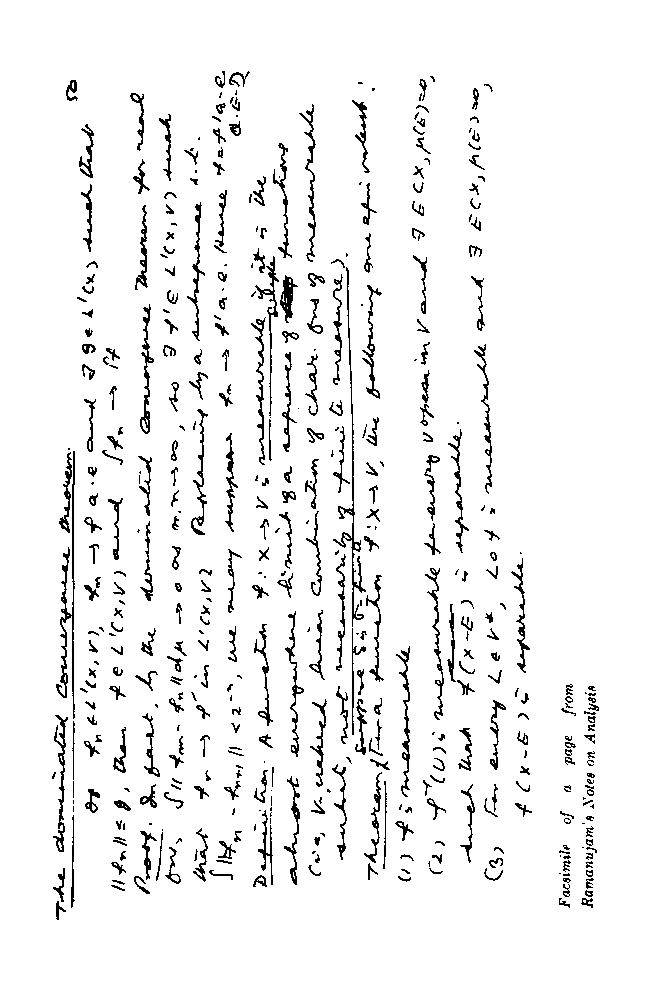
\includegraphics{../017.eps}
\end{figure}

\thispagestyle{empty}

\newpage
~\phantom{a}
\thispagestyle{empty}
